\tikzset{
startstop/.style={rectangle, rounded corners, minimum width=2.5cm, minimum height=0.8cm, text centered, draw=black, fill=red!30},
process/.style={rectangle, minimum width=2.5cm, minimum height=0.8cm, text centered, draw=black, fill=blue!30},
decision/.style={diamond, minimum width=2.5cm, minimum height=0.8cm, text centered, draw=black, fill=green!30},
evaluation/.style={rectangle, rounded corners=0.2cm, minimum width=2.5cm, minimum height=0.8cm, text centered, draw=black, fill=yellow!50},
roundmodel/.style={circle, minimum size=2.0cm, text centered, draw=black, fill=gray!50},
flatgreen/.style={rectangle, rounded corners, minimum width=2.5cm, minimum height=0.8cm, text centered, draw=black, fill=green!50},
purpleblock/.style={rectangle, rounded corners, minimum width=2.5cm, minimum height=0.8cm, text centered, draw=black, fill=purple!50},
arrow/.style={thick,->,>=stealth}
}

\section{Experimental}
This section describes the experimental setup introducing the 3 evaluation setups used to assess the performance of the proposed biometric system and the data splitting strategy used for each evaluation setup.

\subsection{Evaluation Setups}
The evaluation was performed using three distinct types of evaluations:

\begin{itemize}
    \item \textbf{Identification with a Closed Set}: involves including all enrolled patients in the dataset. Each image is classified into one of the known classes (patients) based on its extracted features. The system is trained and tested with the same predefined set of enrolled patients, ensuring no unknown users are present in the dataset.

    \item \textbf{Identification with an Open Set}: excludes a percentage of the enrolled patients from the dataset during training. These excluded patients represent unknown users during the evaluation phase. The model is tested on both known and unknown classes, where the unknown classes are expected to be classified as unknown to simulate open-set identification.

    \item \textbf{Verification}: tests the system's ability to verify the identity of users. Genuine samples consist of images correctly matched to their claimed identities, while imposter samples are created by associating images with incorrect user identities to simulate attempts to mislead the system.
\end{itemize}

\begin{figure}[!ht]
    \centering
    \resizebox{0.7\columnwidth}{!}{
    \begin{tikzpicture}[node distance=1.8cm]
    \node (input) [startstop] {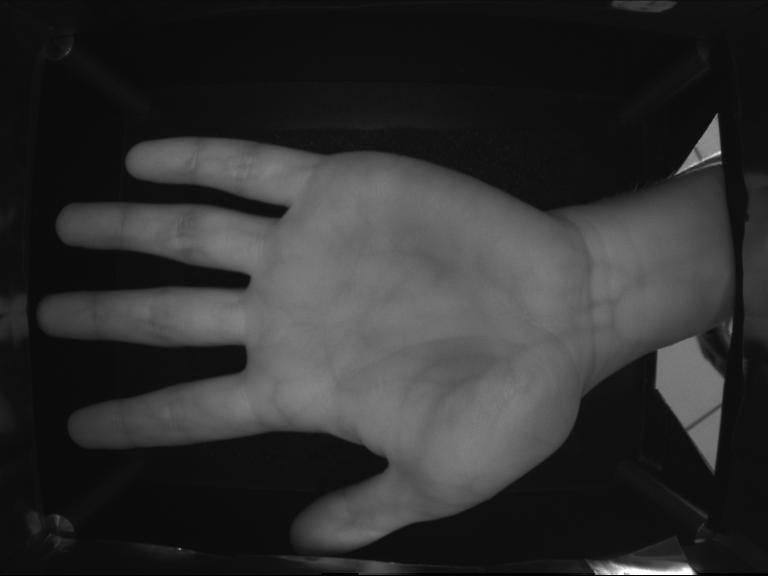
\includegraphics[width=2.5cm]{./images/preprocessing/selected_image.jpg}};
    \node (preprocess) [process, below of=input, yshift=-0.5cm] {Preprocessing};
    \node (binary) [purpleblock, below of=preprocess, yshift=-0.5cm] {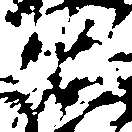
\includegraphics[width=2.5cm]{./images/preprocessing/binarize_image.png}};
    \node (open) [evaluation, below left of=binary, xshift=-2cm, yshift=-1.5cm] {Identification Open};
    \node (closed) [evaluation, below of=binary, yshift=-2cm] {Identification Closed};
    \node (verify) [evaluation, below right of=binary, xshift=2cm, yshift=-1.5cm] {Verification};
    \node (claimed) [startstop, above of=verify, yshift=2cm] {Claimed Identity};
    \node (cnn) [roundmodel, below of=closed, yshift=-1.0cm] {CNN Model};
    \node (output) [flatgreen, below of=cnn, yshift=-0.3cm] {Prediction};
    \draw [arrow] (input) -- (preprocess);
    \draw [arrow] (preprocess) -- (binary);
    \draw [arrow] (binary) -- (open);
    \draw [arrow] (binary) -- (closed);
    \draw [arrow] (binary) -- (verify);
    \draw [arrow] (verify) -- (cnn);
    \draw [arrow] (claimed) -- (verify);
    \draw [arrow] (open) -- (cnn);
    \draw [arrow] (closed) -- (cnn);
    \draw [arrow] (cnn) -- (output);
    \end{tikzpicture}%
    }
    \caption{Experimental Pipeline}
\end{figure}

\subsection{Data Splitting}
To ensure consistent data processing, only images of the left hand were selected from the dataset. This decision was based on the observation that left-hand images generally show fewer imperfections, such as skin damages, which could introduce variability and noise. Additionally, the 850 nm spectrum was chosen for image acquisition. This wavelength was selected because it primarily captures palm vein patterns, avoiding interference from extraneous details such as palm lines that are more visible at the 940 nm spectrum.

The dataset used in this study was split differently for the three evaluation setups:

\textbf{Identification with a Closed Set} includes all patients in the dataset, and their images are divided into training and test sets. The first four images per patient are used for training and the remaining 2 images are used for testing. This setup ensures that all enrolled patients contribute images to the training and testing phases, facilitating evaluation in a controlled, closed-set scenario.

\textbf{Identification with an Open Set} 70\% of patients are randomly selected as known, with their images split into training (first four images) and testing (remaining 2 images). The remaining 30\% serve as unknown patients, with their images used solely for testing to assess the system's ability to handle unenrolled users. 

\textbf{Verification} includes genuine and imposter samples for evaluation. For each patient, the first four images are used for training, and the remaining 2 images are used for testing. Genuine samples consist of matching the correct image to the claimed identity, while imposter samples are created by pairing images from different patients, simulating attempts to impersonate other users. 

To ensure consistency and reproducibility across all splits, a fixed random seed was used during shuffling. This guarantees that the data partitioning remains consistent across different runs and experiments.